\section{Logging impact on performance}

Using standard logging facility is flexible and cost-efficient method for analysing the behaviour of systems like JPaxos.
However, logging takes some CPU time, and therefore may impact results.
Previous JPaxos version used \texttt{java.util.logging} (JUL) for logging, which -- as most built-in Java mechanisms -- is rather performance-unfriendly.
Now JPaxos uses \texttt{slf4j} with \texttt{logback} backend, and two classes of messages are tagged with marks: logging all performance-related events and logging recovery events only.
Slf4j (contrary to java.util.logging) can be turned off at all (i.e. there is no effective logging code). Logback can as well as JUL suppress all messages, makes it however a lot faster.

Tests how much recording events affects performance are presented here:\\
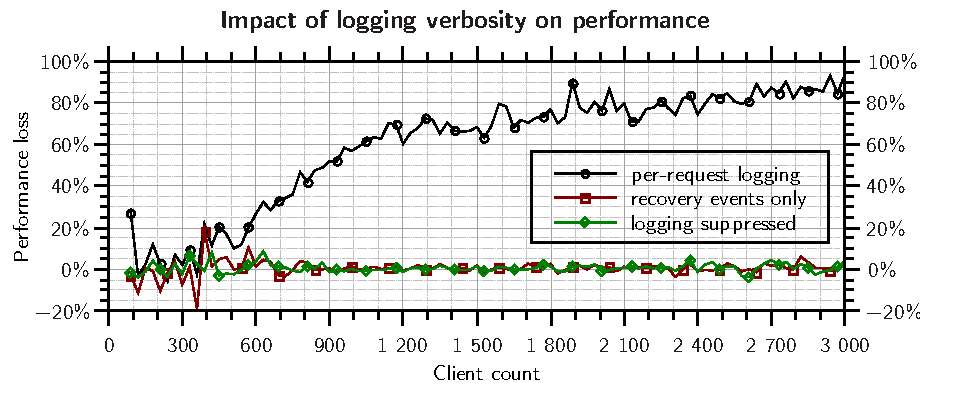
\includegraphics{varia/log_impact.pdf}

Test for each parameter values have been performed once only, however total of 100 tests for different client count are enough to take general conclusions. First, no-op logging is faster than suppressing all logging by 6‰, faster than selecting recovery-related events by 5‰, and faster than logging all performance-related events by 60\%. This means that using logging for recording recovery-related events has little impact on performance and can be used in benchmarks, while full logging on request basis cannot.
Also, full logging cost increases with client count (what is quite obvious, more clients = more requests to trace).
The results for tests up to 900 clients have big variations (what is normal for JPaxos in such case), but the trends remain unaffected.